% !TeX encoding = UTF-8
% !Tex spellcheck = de_DE

%begin:Silbentrennung ****
\RequirePackage{hyphsubst}
\HyphSubstIfExists{ngerman-x-latest}{\HyphSubstLet{ngerman}{ngerman-x-latest}}{} 
\listfiles
%end:Silbentrennung ******

\documentclass[12pt,a4paper]{article}
% ***********************************************************
% ***************** MyStyle - Rene Vollmer*******************
% ***********************************************************
% Version 1.0b



\usepackage[utf8]{inputenc}

\usepackage{hyperref}

\usepackage{amsmath} % AMS Math Package
\usepackage{amsfonts}
\usepackage{amsthm} % Theorem Formatting
\usepackage{amssymb}	% Math symbols such as \mathbb
\usepackage{mathtools}
\usepackage{graphicx} % Allows for eps images
\usepackage{multicol} % Allows for multiple columns
\usepackage[]{units}

\usepackage{hyperref} %Links
\usepackage{url}

\usepackage{verbatim} %Fuer mehrzeilige kommentare \begin{comment} \end{comment}

\usepackage[hang]{caption} % Captions einrücken
\usepackage{subfigure}

%Some other shit
\usepackage{float}
%\floatstyle{boxed} %Puts a box around each figure
\restylefloat{figure}
%\usepackage{wrapfig}
\usepackage{microtype}



\usepackage{xparse} % For uses like \DeclareDocumentCommand{\foocmd}{ O{default1} O{default2} m }{#1~#2~#3}


%\usepackage{color}
%\definecolor{gray}{rgb}{.5,.5,.5}
%\definecolor{lightgray}{rgb}{.25,.25,.25}

%Graphics (PGF / TIKZ) **+**+**+**+**+**+**+**+**+**+**+**+**+**+
\usepackage{tikz}
\usetikzlibrary{patterns}
\tikzset{
	hatchhor/.style={pattern=horizontal lines,pattern color=#1},
	hatchhor/.default=black
}
\tikzset{
	hatchvert/.style={pattern=vertical lines,pattern color=#1},
	hatchvert/.default=black
}
\tikzset{
	hatchdiag/.style={pattern=north east lines,pattern color=#1},
	hatchdiag/.default=black
}
\tikzset{
	hatchdiag2/.style={pattern=north west lines,pattern color=#1},
	hatchdiag2/.default=black
}
%also possible grid, crosshatch, dots, crosshatch dots, fivepointed stars, sixpointed stars

\usepackage{pgfplots}
\usepgfplotslibrary{fillbetween}

% Style to select only points from #1 to #2 (inclusive)
\pgfplotsset{select coords between index/.style 2 args={
		x filter/.code={
			\ifnum\coordindex<#1\def\pgfmathresult{}\fi
			\ifnum\coordindex>#2\def\pgfmathresult{}\fi
		}
	}
}


\newcommand{\vasymptote}[2][]{
	\draw [color=gray,densely dashed,#1] ({rel axis cs:0,0} -| {axis cs:#2,0}) -- ({rel axis cs:0,1} -| {axis cs:#2,0});
}

\newcommand{\vertline}[2][]{
	\draw [#1] ({rel axis cs:0,0} -| {axis cs:#2,0}) -- ({rel axis cs:0,1} -| {axis cs:#2,0});
}
%END Graphics **+**+**+**+**+**+**+**+**+**+**+**+**+**+**+**+**+

%Stolen from http://www.dfcd.net/articles/latex/latex.html
% **#**#**#**#**#**#**#**#**#**#**#**#**#**#**#**#**#**#**#**#**#
\makeatletter % Need for anything that contains an @ command

\let\vaccent=\v % rename builtin command \v{} to \vaccent{}
\renewcommand{\v}[1]{\ensuremath{\mathbf{#1}}} % for vectors
\newcommand{\gv}[1]{\ensuremath{\mbox{\boldmath$ #1 $}}} 
% for vectors of Greek letters
\newcommand{\uv}[1]{\ensuremath{\mathbf{\hat{#1}}}} % for unit vector
\newcommand{\abs}[1]{\left| #1 \right|} % for absolute value
\newcommand{\avg}[1]{\left< #1 \right>} % for average
\let\underdot=\d % rename builtin command \d{} to \underdot{}
\renewcommand{\d}[2]{\frac{d #1}{d #2}} % for derivatives
\newcommand{\niced}[2]{\nicefrac{d #1}{d #2}} % for in-text-derivatives
\newcommand{\nicedd}[2]{\nicefrac{d^2 #1}{d #2^2}} % for double derivatives\newcommand{\dd}[2]{\frac{d^2 #1}{d #2^2}} % for in-text-double derivatives
\newcommand{\pd}[2]{\frac{\partial #1}{\partial #2}} 
% for partial derivatives
\newcommand{\pdd}[2]{\frac{\partial^2 #1}{\partial #2^2}} 
% for double partial derivatives
\newcommand{\pdc}[3]{\left( \frac{\partial #1}{\partial #2}
	\right)_{#3}} % for thermodynamic partial derivatives
\newcommand{\ket}[1]{\left| #1 \right>} % for Dirac bras
\newcommand{\bra}[1]{\left< #1 \right|} % for Dirac kets
\newcommand{\braket}[2]{\left< #1 \vphantom{#2} \right|
	\left. #2 \vphantom{#1} \right>} % for Dirac brackets
\newcommand{\matrixel}[3]{\left< #1 \vphantom{#2#3} \right|
	#2 \left| #3 \vphantom{#1#2} \right>} % for Dirac matrix elements
\newcommand{\grad}[1]{\gv{\nabla} #1} % for gradient
\let\divsymb=\div % rename builtin command \div to \divsymb
\renewcommand{\div}[1]{\gv{\nabla} \cdot #1} % for divergence
\newcommand{\curl}[1]{\gv{\nabla} \times #1} % for curl
\let\baraccent=\= % rename builtin command \= to \baraccent
\renewcommand{\=}[1]{\stackrel{#1}{=}} % for putting numbers above =
\newtheorem{prop}{Proposition}
\newtheorem{thm}{Theorem}[section]
\newtheorem{lem}[thm]{Lemma}
\theoremstyle{definition}
\newtheorem{dfn}{Definition}
\theoremstyle{remark}
\newtheorem*{rmk}{Remark}
% **#**#**#**#**#**#**#**#**#**#**#**#**#**#**#**#**#**#**#**#**#


%Equalssign with hat/corresponds to   \equalhat
\newcommand\equalhat{%
	\stackrel{\Lambda}{=}
}
%Equalssign with !
\newcommand\shallbe{%
	\stackrel{!}{=}
}
% := and =:
\newcommand{\defeq}{\vcentcolon=}
\newcommand{\eqdef}{=\vcentcolon}



%Encirecled Numbers, used in Graphics
\let\depth\relax
\def\X#1{%
	%#1%
	%\textcircled{#1}%
	\raisebox{0.9pt}{\textcircled{\raisebox{-.9pt}{#1}}}%
	%\ding{\numexpr171+#1\relax}%
}


% ******************************~~~~*****************************
%Photo quality management. This is an old try:
\newcommand\openfile{\newwrite\outputstream\immediate\openout\outputstream=photo.log
	\writetofile[linewidth]{\the\linewidth}
	\writetofile[textwidth]{\the\textwidth}
	\writetofile[dpi]{300}
	}
\newcommand\closefile{\immediate\closeout\outputstream}
\newcommand\writetofile[2][2]{\immediate\write\outputstream{#1 #2}}

\newcommand\photo[2][2]{\includegraphics[width=#1]{#2}\writetofile[#2]{#1}}

% ***************************************************************
% And this is working
% Reduce image size for fixed dpi
% Introduce \includegraphicsRS for this purpose

% for downsampling large images: \includegraphicsRS
% (\includegraphics "resize")
% \includegraphicsRS[#1][#2]{#3}
% #1 = normal \includegraphics[] - Parameter (like scale=1) {optional}
% #2 = approx part of the screen, eg half page width use 0.5 or 1/2 {optional}
%      reduces to #2*1000px
% #3 = relative path to image file WITH ending (e.g. .jpg) {required}
\pdfimageresolution 300

\newcommand{\includegraphicsRS}{}

\ifnum\pdfshellescape=1
% Yes, enabled
% IFP - image file path
% IFN - image filename only
% here resizing at #2*1000 px wide
\newread\myinput
% must add default argument [] so typeout works
\DeclareDocumentCommand{\includegraphicsRS}{ O{\@empty} O{1} m }{ %
%\renewcommand\includegraphicsRS[2][\@empty]{
	% run downsampling bash script
	\immediate\write18{mkdir -p images; mkdir -p images/downsampled; IFP=#3 ; %
		PIX=#2 ; PIX=$( awk  'BEGIN { rounded = sprintf("\%.0f", ('$PIX')*1000); print rounded }' ) ;
		echo "$PIX 1000 *p" | dc ; %
		echo "Processing $IFP" ; %
		IFN=$(basename $IFP) ; %
		echo "images/downsampled/$IFN" > tmpname ; %
		if [ ! -f images/downsampled/$IFN ]; then %
		echo "File images/downsampled/$IFN not found! Converting..." ; %
		%the \string> after the pixel width (e.g. 1000x) will prevent imagemagick from producing files larger than the original
		convert $IFP -resize $PIX"x\string>" -quality 85 images/downsampled/$IFN ; %

		else %
		echo "Found images/downsampled/$IFN - reusing." ; %
		fi ; %
		%alternatively: bash includegraphicsRS.sh #3 #2
		%and have the code in the *.sh-file.
	} % end write18
	% here we should have downsampled file
	% retrieve downsample filename first
	\immediate\openin\myinput=tmpname
	% The group localizes the change to \endlinechar
	\bgroup
	\endlinechar=-1
	\immediate\read\myinput to \localline
	% Since everything in the group is local, we have to explicitly make the
	% assignment global
	\global\let\myTmpFileName\localline
	\egroup
	\immediate\closein\myinput
	% Clean up after ourselves
	% \immediate\write18{rm -f -- tmpname}
	% finally, include downsampled image
	\includegraphics[#1]{\myTmpFileName}
} % end renewcommand
\else
% No, disabled
% in this case, \includegraphicsRS is just the usual \includegraphics
\renewcommand\includegraphicsRS[2][\@empty]{%
	\includegraphics[#1]{#2}
}
\fi

\begin{comment}
old stuff, not used any longer. Could be useful for future changes though.
\usepackage{fp}

\newlength{\TOarg} \newlength{\TOunit}
{\catcode`p=12 \catcode`t=12 \gdef\TOnum#1pt{#1}}
\newcommand\TOop[2]{\setlength{\TOarg}{#2}%
	\FPdiv\TOres{\expandafter\TOnum\the\TOarg}{\expandafter\TOnum\the\TOunit}%
	\FPround\TOres\TOres{#1}}
\newcommand{\TOspace}{\ }
\newcommand\TOpt[2][2]{\setlength{\TOunit}{1pt}\TOop{#1}{#2}\TOres\TOspace pt}
\newcommand\TOin[2][2]{\setlength{\TOunit}{1in}\TOop{#1}{#2}\TOres\TOspace in}
\newcommand\TOcm[2][2]{\setlength{\TOunit}{1cm}\TOop{#1}{#2}\TOres\TOspace cm}
\newcommand\TOmm[2][2]{\setlength{\TOunit}{1mm}\TOop{#1}{#2}\TOres\TOspace mm}
\newcommand\TOem[2][2]{\setlength{\TOunit}{1em}\TOop{#1}{#2}\TOres\TOspace em}
\newcommand\TOpx[2][2]{\setlength{\TOunit}{1px}\TOop{#1}{#2}\TOres\TOspace px}
\newcommand\TOptdeux[2][2]{\setlength{\TOunit}{1pt}\TOop{#1}{#2}\TOres}

convert $IFP -resize 50\% images/downsampled/$IFN ; %		textwidth="\the\textwidth" ; %
TW=${textwidth:0:(-2)} ; %
VARI="$TW"; %
convert -resize 2000x -units pixelspercentimeter $IFP -density 120 -pointsize 30 -draw "gravity south-east fill black text 0,5 '$VARI'" downsampled/$IFN ; %
\end{comment}


% END of \includegraphicsRS
% ***************************************************************
% ******************************~~~~*****************************



% ***********************************************************
% ********************** END HEADER *************************
% ***********************************************************
\usepackage[left=2.50cm, right=2.50cm, top=2.50cm, bottom=2.00cm]{geometry}

%test
\begin{comment}
\usepackage{titlesec}
\titleformat{\subsection}[runin]% runin puts it in the same paragraph
{\normalfont\bfseries}% formatting commands to apply to the whole heading
{\thesubsection}% the label and number
{0.5em}% space between label/number and subsection title
{}% formatting commands applied just to subsection title
[]% e.g. [.] punctuation or other commands following subsection title\frac{•}{•}
\end{comment}


\linespread{1.1}
\usepackage{microtype}

%\addto\captionsgerman{ \renewcommand{\figurename}{\small{\textbf{Abb.}}}
%\captionsetup{figurewithin = section}
%\captionsetup{font=small, labelfont=bf} }


\begin{document}
	
	\pagenumbering{Roman}
	%TODO REMOVE
	\textbf{TODO}
	
René
\begin{enumerate}
	\item Regina sagen, dass sie auf die Eigenschaften der FT refen soll
	\item Regine Videos vom Handy geben
	\item Regina Rücktransformierte Bilder geben
	\item 
\end{enumerate}

Vivi
\begin{enumerate}
	\item @ rené: ich hab bei der section "einkopplung" jetzt keine unsrer Leistungs-berechnungs- rechnungen hingeschrieben, weil die ja alle für die photodiode waren, mit irgendwelchen zu großen widerständen... 
	\item ...
\end{enumerate}
	
	
	%Metadaten
	\title{\textit{Fortgeschrittenenpraktikum}\\\textbf{Quantenhalleffekt} }
	\date{September 2015}
	\author{Vivien Sleziona \footnote{vivi.s@arcor.de}\\ René Vollmer \footnote{rene.vollmer@studium.uni-hamburg.de} \\ \\Betreut durch\\ Nils Gayer\footnote{ngayer@physnet.uni-hamburg.de}}
	
	\maketitle
	
	\begin{center} 
		\bigskip
		\bigskip
		
		\begin{minipage}{0.75\textwidth}
			% !TeX root = ../praktikum.tex
% !TeX encoding = UTF-8
% !Tex spellcheck = de_DE

Die Fourier-Analytik und insbesondere die Fouriertransformation sind auf vielen modernen Anwendungen kaum noch weg zu denken. Sie ist essentieller Bestandteil vieler Bildverarbeitungsalgorithmen\cite{easton_fourier_2010} und -kompressionsverfahren wie JPEG\cite{_jpeg_2015}, sie wird genutzt um Bildinformationen Computeralgorithmen zugänglich zu machen\cite{prof._dr._norbert_link_vorlesungsscript:_????} und in vielen anderen Bereichen der Signalverarbeitung.\\

In diesem Versuch soll mit einfachen optischen Mitteln eine Fouriertransformation auf Bildern durchgeführt, die Fouriertransformierte manipuliert und rücktransformiert werden. Dabei wird dem Leser ein intuitives Verständnis für die Funktionsweise und Bedeutung von Fouriertransformationen vermittelt werden.
		\end{minipage}
	\end{center}
	
	%\vfill
	\newpage
	
	\tableofcontents
	\vfill
	\newpage
	\clearpage	
	
	\pagenumbering{arabic}
	
	\section{Theoretische Grundlagen}
	
	% !TeX root = ../praktikum.tex
% !TeX encoding = UTF-8
% !Tex spellcheck = de_DE

\begin{align}
	\vec{\j} = \mathbf{\sigma} \cdot \vec{E} & & \Leftrightarrow & & \vec{E} = \mathbf{\rho} \cdot \vec{j}
	\label{eq:u2rho}
\end{align}

	
	\newpage
	\clearpage
	
	\section{Experimentelle Durchführung und Beobachtungen}
	Der Versuchsaufbau besteht aus einem im Boden eingelassenen Kryostaten und sich in einem Rack befindlicher Steuerungs- und Messelektronik, welche mit Hilfe eines Computers gesteuert bzw. ausgelesen und aufgezeichnet werden kann. Der Kryostat ist ein Vakuumtank mit einer heliumgefüllten Kammer im Inneren. Darin befindet sich ein Probeneinschub. Mit einer Pumpe wird der Druck in diesem auf wenigen Millibar gehalten. Durch die Verdunstungskälte kann die Innentemperatur auf unter \unit[1,5]{K} gehalten werden.
	
	Für den Versuch wird als erstes die Probe an der Spitze eines Stabes montiert und in den Probeneinschub eingeführt. Anschließend wird dieser mehrfach mit Helium geflutet und abgepumpt, um Luftreste zu entfernen und Vereisungen zu vermeiden. Bei laufender Pumpe wird eine Einstellung für die Heliumzufuhr gesucht, sodass sich in dem Probeneinschub der gewünschte Druck einstellt.\\
	
	Im Nachfolgenden werden in den ersten beiden Abschnitten zwei unterschiedliche Messmethoden erprobt und in den anschließenden werden Winkel, Temperatur und Elektronendichte verändert und die Folgen auf den Quanten-Hall Effekt und die Shubnikov-de Haas Oszillationen untersucht.
	
	\subsection{Gleichstrommessungen}
	\label{ch:dc}
	% !TeX root = ../praktikum.tex
% !TeX encoding = UTF-8
% !Tex spellcheck = de_DE

In diesem Versuchsabschnitt werden die beiden zu untersuchenden Effekte gemessen, während an der Probe ein Gleichstrom anliegt. Hierzu wird gleichzeitig der Spannungsabfall über die Länge und über die Breite der Probe mit der Software erfasst. An die Probe wird in x-Richtung ein konstanter Gleichstrom von $\unit[1]{\mu A}$ angelegt. Um eine stabile Temperatur zu erhalten, wurde die Kammer auf \unit[2]{K} geheizt. Jetzt wurde das Magnetfeld auf \unit[-7]{T} gefahren. Dies dauert rund sieben Minuten, da es sich um supraleitende Spulen handelt und das Anlegen eines Stroms eine Gegeninduktion verursacht. Sobald das Magnetfeld aufgebaut ist, wird die Hallspannung $U_H$ sowie die Längsspannung $U_{xx}$ aufgezeichnet, während das Magnetfeld mit etwa \unitfrac[1]{T}{min} auf \unit[7]{T} gefahren wird. 


Diese Messdaten sind zusammen mit einer weiteren Messung im Bereich von $-2$ bis \unit[+2]{T} bei einer konstanten Erhöhung von \unitfrac[0,2]{T}{min} in Abbildung~\ref{fig:full_range_dc} aufgetragen.

\begin{figure}[h]
	\centering
	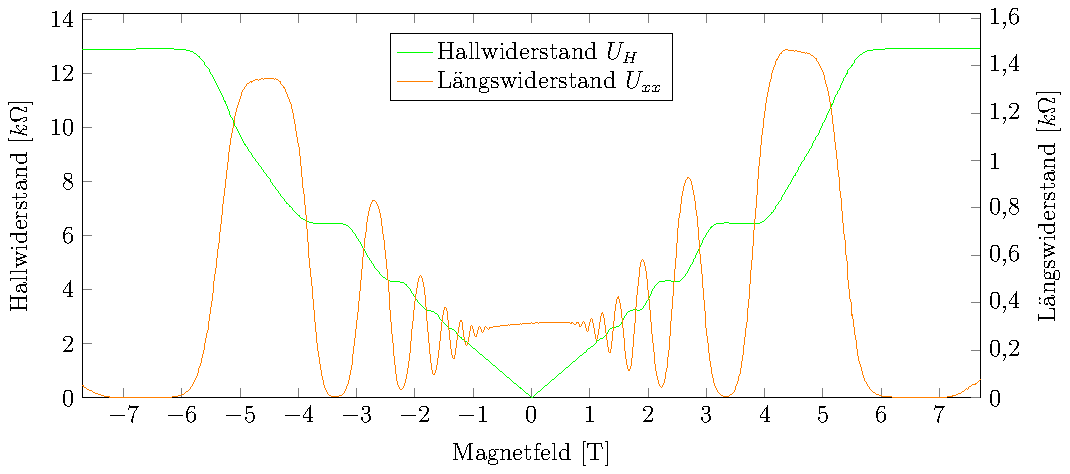
\includegraphics{graphs/dc/full_range.pdf}
	\caption[Gleichstrommessung im maximalen Magnetfeldbereich]{
		Hall-Widerstand und Shubnikov-de Haas Oszillationen eines mit Gleichstrom durchflossenen 2DES.
	}
	\label{fig:full_range_dc}
\end{figure}

Es sind deutlich die Plateaus des Hall- und Shubnikov-de Haas-Widerstandes zu erkennen.


\begin{figure}[h]
	\centering
	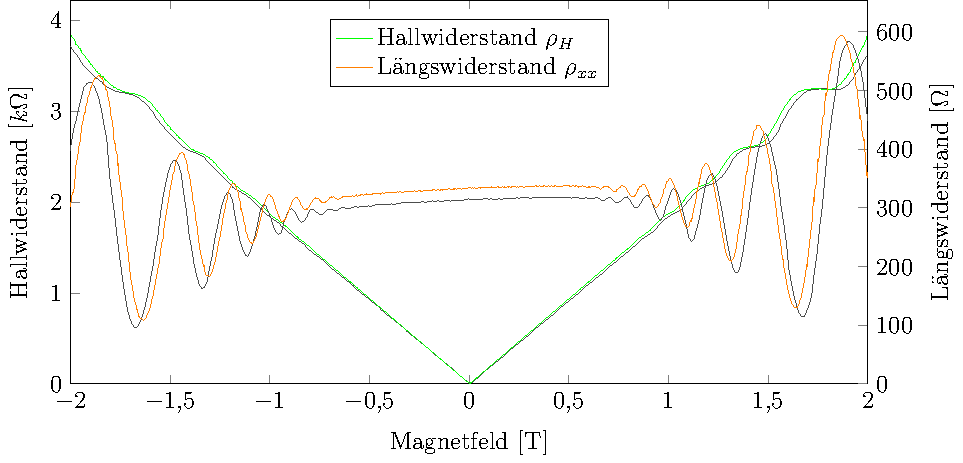
\includegraphics{graphs/dc/pm2T_range.pdf}
	\caption[Höher aufgelöste Gleichstrommessung in Magnetfeldteilbereich]{
		Hall-Widerstand und Shubnikov-de Haas Oszillationen eines mit Gleichstrom durchflossenen 2DES.
	}
	\label{fig:2T_range_dc}
\end{figure}
	\subsection{Wechselstrommessung}
	\label{ch:ac}
	% !TeX root = ../praktikum.tex
% !TeX encoding = UTF-8
% !Tex spellcheck = de_DE

Im folgendem Abschnitt wurden die Messungen des vorigen Versuchsteils im Wesentlichen wiederholt, mit dem Unterschied, dass anstatt eines Gleichstroms ein Wechselstrom angelegt %TODO: Spannung oder SStrom?! 
 %mit $U_{RMS}=\unit[1]{V}$ angelegt wurde und ein \unit[9,95]{$M\Omega$} Widerstand in Reihe geschaltet wurde. 
 Um einen Wechselstrom erzeugen zu können, wurden sogenannte Lock-in Verstärker genutzt. Ein Lock-in Verstärker enthält einen Funktionsgenerator, welcher anhand einer einstellbaren Frequenz eine sinusförmige Wechselspannung mit $U_{RMS}=\unit[1]{V}$ ausgibt. Um den Strom unabhängig von dem Widerstand des Hall-Streifens zu halten, musste ein hinreichend großer Widerstand in Reihe geschaltet werden. Da der Eigenwiderstand des Hall-Streifens bei einigen Megaohm lag, wurde ein  \unit[9,95]{$M\Omega$} Widerstand verwendet. So kann in guter Näherung angenommen werden, dass der Strom allein durch den zusätzlich angelegten Vorwiderstand zu $I=\nicefrac{U}{R}=\nicefrac{\unit[1]{V}}{\unit[9,95]{M\Omega}}=\unit[0,995]{\mu A}$ bestimmt wurde. 
 Bei der Durchführung der Wechselstrommessung fiel auf, dass die Plateaus im Graphen der Hallspannung %TODO: Hallwiderstand?
 deutlich ausgeprägter ausfielen, als für die Gleichstrommessung. Analog dazu waren hier schmalere Peaks in der Shubnikov-de Haas-Oszillation zu erkennen.  
 Erneut konnte die Formel~\eqref{eq:u2rho} genutzt werden, um den Widerstand aus dem Spannungsabfall zu erhalten. %TODO: Hallwiderstand?

\begin{figure}[h]
	\centering
	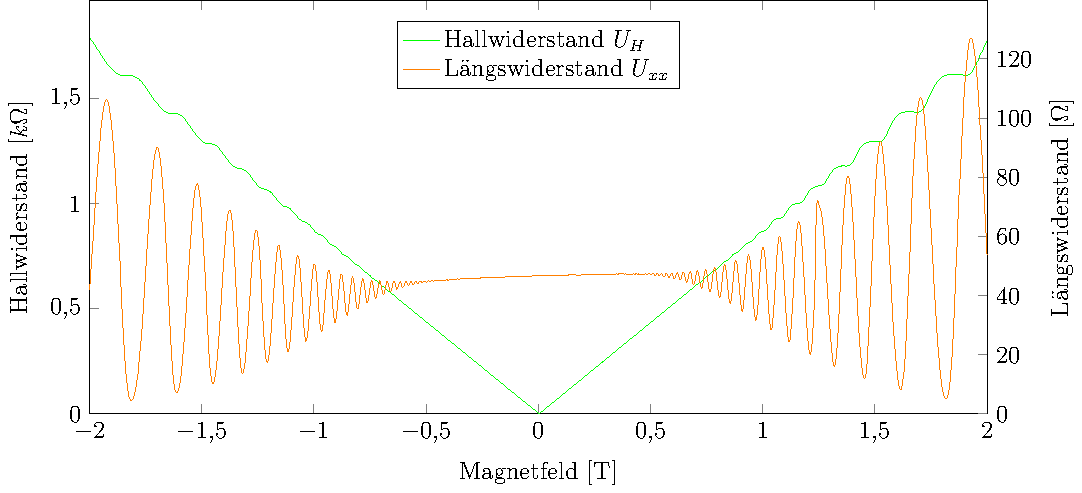
\includegraphics{graphs/ac/pm2T_range.pdf}
	\caption[Höher aufgelöste Gleichstrommessung in Magnetfeldteilbereich]{
		Hall-Widerstand und Shubnikov-de Haas Oszillationen eines mit Gleichstrom durchflossenen 2DES.
	}
	\label{fig:2T_range_ac}
\end{figure}


\begin{figure}[h]
	\centering
	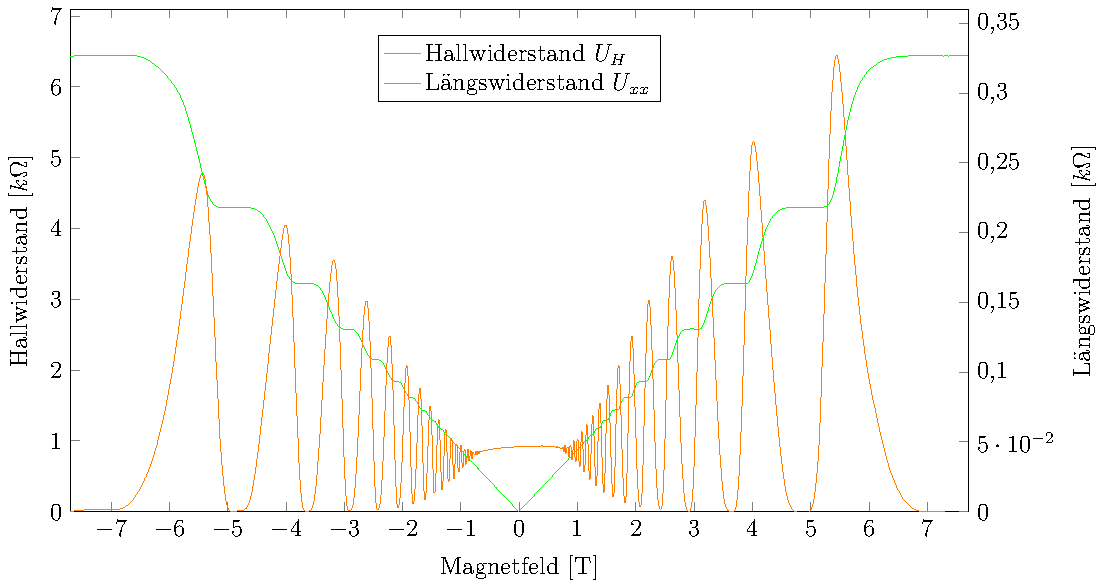
\includegraphics{graphs/ac/full_range.pdf}
	\caption[Wechselstrommessung im maximalen Magnetfeldbereich]{
		Hall-Widerstand und Shubnikov-de Haas Oszillationen eines mit Wechselstrom durchflossenen 2DES.
	}
	\label{fig:full_range_ac}
\end{figure}



	\subsection{Winkelabhängigkeit}
	\label{ch:winkel}
	% !TeX root = ../praktikum.tex
% !TeX encoding = UTF-8
% !Tex spellcheck = de_DE

In diesem Versuchsteil wurde die Abhängigkeit des Quanten-Hall-Effekts, sowie des Shubnikov-de Haas-Effekts vom Einfallswinkel des Magnetfeldes auf die Probe untersucht. Hierzu wurde ausgenutzt, dass sich der Probenstab im Einschub drehen ließ, ohne sich dabei aus der Fixierung zu lösen. 
Mit Hilfe einer Winkelscheibe auf der Abdeckung des Kryostaten und einer Markierung am Probenstab, wurde nun eine Messreihe bestehend aus mehreren Messungen für verschiedene Winkeleinstellungen der Probe zum Magnetfeld durchgeführt. Für den Winkel wurden hierbei in $10^\circ$-Schritten Werte zwischen $260^\circ$ und $10^\circ$  gewählt, sodass insgesamt eine Drehung von $110^\circ$ ausgeführt wurde. Dabei lag eine Temperatur von \unit[2]{K} an der Probe an und für jede Messung wurde das Magnetfeld analog zu den ersten Messungen von $+7,7$ bis \unit[-7,7]{T} gefahren, mit der maximalen Geschwindigkeit von \unitfrac[1]{T}{min}. Aufgrund der deutlicheren Hall-Plateaus in den Graphen wurde für diese Messreihe weiterhin die Wechselstromquelle des vorangegangenen Versuchsteils genutzt. 

Anhand der Messungen war zu erkennen, dass beide betrachteten Effekte immer weniger ausgeprägt waren und schließlich verschwanden, je weiter die Probe aus der Nullposition ausgelenkt wurde. 
	\subsection{Temperaturabhängigkeit}
	\label{ch:temp}
	% !TeX root = ../praktikum.tex
% !TeX encoding = UTF-8
% !Tex spellcheck = de_DE

Im Folgenden sollte nun die Temperaturabhängigkeit des Quanten-Hall- und des Shubnikov-de Haas-Effekts überprüft werden. Ziel dabei war es, die Grenztemperatur zu finden, bis zu welcher die beiden Effekte noch zu beobachten sind. 
Dazu wurden Messungen für unterschiedliche Temperaturwerte an der Probe aufgenommen. Begonnen wurde dabei bei der Ausgangstemperatur von \unit[2]{K} und es wurden in unregelmäßigen Intervallen Temperaturen bis hin zu \unit[40]{K} gewählt. Für jede Messung wurde analog zu den vorangegangenen Versuchsteilen das Magnetfeld mit einer Geschwindigkeit von \unitfrac[1]{T}{min} hochgefahren, diesmal von jeweils 0 bis \unit[7]{T}. Auch hier wurde aufgrund der deutlicheren Hall-Plateaus in den Graphen weiterhin die Wechselstromquelle genutzt. 

Wie aus den Graphen %TODO: Graphen
ersichtlich, liegt die gesuchte Grenztemperatur, bis zu welcher der Quanten-Hall- und der Shubnikov-de Haas-Effekt noch zu beobachten sind, bei etwa \unit[15]{K}. %TODO: richtiger Wert?






	\subsection{Gatespannungsabhängigkeit}
	\label{ch:gate}
	% !TeX root = ../praktikum.tex
% !TeX encoding = UTF-8
% !Tex spellcheck = de_DE

Im letzten Versuchsabschnitt wurde der Einfluss einer Gatespannung auf die beiden zu untersuchenden Effekte beleuchtet, mit dem Ziel, aus den dadurch erfassten Daten, den Abstand des 2DEG in der Probe zur Gateelektrode zu bestimmen. Generell kann das Anlegen einer Gatespannung den Bandverlauf in der Probe verändern. % WAS IST EINE GATESPANNUNG?
Die Position der Gateelektrode an der Probe ist aus Abbildung %TODO: Schema der Probe
ersichtlich. 
Für die folgenden Messungen wurden in Schritten von \unit[50]{mV} Gatespannungen von -200 bis \unit[200]{mV} gewählt.
Dabei wurde eine Temperatur von \unit[2]{K} an der Probe eingestellt und analog zu den obigen Versuchsteilen aufgrund der deutlicheren Hall-Plateaus in den Graphen die Wechselstromquelle genutzt. 






	
	\newpage
	\clearpage
	
	\section{Auswertung}
	\label{chap:auswertung}
	% !TeX encoding = UTF-8
% !TeX spellcheck = de_DE

\documentclass[12pt,border=0mm]{standalone}


\usepackage[utf8]{inputenc}

\usepackage{hyperref}

\usepackage{amsmath} % AMS Math Package
\usepackage{amsfonts}
\usepackage{amsthm} % Theorem Formatting
\usepackage{amssymb}	% Math symbols such as \mathbb
\usepackage{mathtools}
\usepackage{graphicx} % Allows for eps images
\usepackage{multicol} % Allows for multiple columns
\usepackage[]{units}

\usepackage{hyperref} %Links
\usepackage{url}

\usepackage{verbatim} %Fuer mehrzeilige kommentare \begin{comment} \end{comment}

\usepackage[hang]{caption} % Captions einrücken
\usepackage{subfigure}

%Some other shit
\usepackage{float}
%\floatstyle{boxed} %Puts a box around each figure
\restylefloat{figure}
%\usepackage{wrapfig}
\usepackage{microtype}



\usepackage{xparse} % For uses like \DeclareDocumentCommand{\foocmd}{ O{default1} O{default2} m }{#1~#2~#3}

%\usepackage{color}
%\definecolor{gray}{rgb}{.5,.5,.5}
%\definecolor{lightgray}{rgb}{.25,.25,.25}

%Graphics (PGF / TIKZ) **+**+**+**+**+**+**+**+**+**+**+**+**+**+
\usepackage{tikz}
\usetikzlibrary{patterns}
\tikzset{
	hatchhor/.style={pattern=horizontal lines,pattern color=#1},
	hatchhor/.default=black
}
\tikzset{
	hatchvert/.style={pattern=vertical lines,pattern color=#1},
	hatchvert/.default=black
}
\tikzset{
	hatchdiag/.style={pattern=north east lines,pattern color=#1},
	hatchdiag/.default=black
}
\tikzset{
	hatchdiag2/.style={pattern=north west lines,pattern color=#1},
	hatchdiag2/.default=black
}
%also possible grid, crosshatch, dots, crosshatch dots, fivepointed stars, sixpointed stars

\usepackage{pgfplots}
\usepgfplotslibrary{fillbetween}

% Style to select only points from #1 to #2 (inclusive)
\pgfplotsset{select coords between index/.style 2 args={
		x filter/.code={
			\ifnum\coordindex<#1\def\pgfmathresult{}\fi
			\ifnum\coordindex>#2\def\pgfmathresult{}\fi
		}
	}
}


\newcommand{\vasymptote}[2][]{
	\draw [color=gray,densely dashed,#1] ({rel axis cs:0,0} -| {axis cs:#2,0}) -- ({rel axis cs:0,1} -| {axis cs:#2,0});
}

\newcommand{\vertline}[2][]{
	\draw [#1] ({rel axis cs:0,0} -| {axis cs:#2,0}) -- ({rel axis cs:0,1} -| {axis cs:#2,0});
}
%END Graphics **+**+**+**+**+**+**+**+**+**+**+**+**+**+**+**+**+
%Stolen from http://www.dfcd.net/articles/latex/latex.html
% **#**#**#**#**#**#**#**#**#**#**#**#**#**#**#**#**#**#**#**#**#
\makeatletter % Need for anything that contains an @ command

\let\vaccent=\v % rename builtin command \v{} to \vaccent{}
\renewcommand{\v}[1]{\ensuremath{\mathbf{#1}}} % for vectors
\newcommand{\gv}[1]{\ensuremath{\mbox{\boldmath$ #1 $}}} 
% for vectors of Greek letters
\newcommand{\uv}[1]{\ensuremath{\mathbf{\hat{#1}}}} % for unit vector
\newcommand{\abs}[1]{\left| #1 \right|} % for absolute value
\newcommand{\avg}[1]{\left< #1 \right>} % for average
\let\underdot=\d % rename builtin command \d{} to \underdot{}
\renewcommand{\d}[2]{\frac{d #1}{d #2}} % for derivatives
\newcommand{\niced}[2]{\nicefrac{d #1}{d #2}} % for in-text-derivatives
\newcommand{\nicedd}[2]{\nicefrac{d^2 #1}{d #2^2}} % for double derivatives\newcommand{\dd}[2]{\frac{d^2 #1}{d #2^2}} % for in-text-double derivatives
\newcommand{\pd}[2]{\frac{\partial #1}{\partial #2}} 
% for partial derivatives
\newcommand{\pdd}[2]{\frac{\partial^2 #1}{\partial #2^2}} 
% for double partial derivatives
\newcommand{\pdc}[3]{\left( \frac{\partial #1}{\partial #2}
	\right)_{#3}} % for thermodynamic partial derivatives
\newcommand{\ket}[1]{\left| #1 \right>} % for Dirac bras
\newcommand{\bra}[1]{\left< #1 \right|} % for Dirac kets
\newcommand{\braket}[2]{\left< #1 \vphantom{#2} \right|
	\left. #2 \vphantom{#1} \right>} % for Dirac brackets
\newcommand{\matrixel}[3]{\left< #1 \vphantom{#2#3} \right|
	#2 \left| #3 \vphantom{#1#2} \right>} % for Dirac matrix elements
\newcommand{\grad}[1]{\gv{\nabla} #1} % for gradient
\let\divsymb=\div % rename builtin command \div to \divsymb
\renewcommand{\div}[1]{\gv{\nabla} \cdot #1} % for divergence
\newcommand{\curl}[1]{\gv{\nabla} \times #1} % for curl
\let\baraccent=\= % rename builtin command \= to \baraccent
\renewcommand{\=}[1]{\stackrel{#1}{=}} % for putting numbers above =
\newtheorem{prop}{Proposition}
\newtheorem{thm}{Theorem}[section]
\newtheorem{lem}[thm]{Lemma}
\theoremstyle{definition}
\newtheorem{dfn}{Definition}
\theoremstyle{remark}
\newtheorem*{rmk}{Remark}
% **#**#**#**#**#**#**#**#**#**#**#**#**#**#**#**#**#**#**#**#**#


%Equalssign with hat/corresponds to   \equalhat
\newcommand\equalhat{%
	\stackrel{\Lambda}{=}
}
%Equalssign with !
\newcommand\shallbe{%
	\stackrel{!}{=}
}
% := and =:
\newcommand{\defeq}{\vcentcolon=}
\newcommand{\eqdef}{=\vcentcolon}



%Encirecled Numbers, used in Graphics
\let\depth\relax
\def\X#1{%
	%#1%
	%\textcircled{#1}%
	\raisebox{0.9pt}{\textcircled{\raisebox{-.9pt}{#1}}}%
	%\ding{\numexpr171+#1\relax}%
}

% Style to select only points from #1 to #2 (inclusive)
\pgfplotsset{select coords between index/.style 2 args={
		x filter/.code={
			\ifnum\coordindex<#1\def\pgfmathresult{}\fi
			\ifnum\coordindex>#2\def\pgfmathresult{}\fi
		}
	}}
	
	

\usepackage{pgfplots}
\usepackage{tikz}

\usepgfplotslibrary{smithchart}
%\usepgfplotslibrary[smithchart]
%\usetikzlibrary{pgfplots.smithchart}
%\usetikzlibrary[pgfplots.smithchart]
\pgfplotsset{compat=1.12}

%a4: width=21.00cm, height=29.70cm
%borders 2.5cm each side => width=16.00cm*0.95=15.2cm
%\usepackage[left=2cm, right=1cm, top=1cm, bottom=1cm]{geometry}

\usepackage{pgfplotstable}
\def\probelength{600} %µm
\def\probewidth{100} %µm
\def\probecurrent{(-(\thisrowno{5})*10^6)} %µA
\def\unitfactor{10^3} %
\def\UhallEq{(abs(\thisrowno{1})/\probecurrent)*\unitfactor}
\def\UxxEq{\thisrowno{4}*\probewidth/(\probelength*\probecurrent)*\unitfactor} %kOhm


\begin{document}
	
	\begin{tikzpicture}
	
	\begin{axis}[
		%axis y line*=left,
		width=15.2cm, height=7cm,
		xmin=-2,xmax=2, %ymin=0, %ymax=14,
		xlabel={Reziprokes Magnetfeld \nicefrac{1}{B} [${T}^{-1}$]},
		ylabel={Füllfaktor [$\nu$]},
		legend pos=north west,
	]
	
		%\addplot[mark=x, only marks] table[x index=1, y index=3] {../data/wechselspannung/ausgewertet.dat};
		
		%\vertline{0.5}
		%\vertline{-0.5}
		
		\addplot[mark=x, only marks] table[select coords between index={5}{36}, x index=1, y index=3] {../data/wechselspannung/ausgewertet.dat};
		\addlegendentry{SDHO mit Minima $\rho_{xx}\neq 0$}
		
		\addplot[mark=o, only marks, forget plot] table[select coords between index={0}{4}, x index=1, y index=3] {../data/wechselspannung/ausgewertet.dat};
		\addplot[mark=o, only marks] table[select coords between index={37}{43}, x index=1, y index=3] {../data/wechselspannung/ausgewertet.dat};
		\addlegendentry{SDHO mit Minima $\rho_{xx}=0$}
		%\addlegendentry{$U_H$}
		
		\addplot[red, mark=\empty] {x*28.9081133643839};
		\addlegendentry{Lineare Regression }
		
		%\addplot table[x index=1, y={create col/linear regression={y=C3}}] {../data/wechselspannung/ausgewertet.dat};\addlegendentry{%
		%	$\pgfmathprintnumber{\pgfplotstableregressiona} \cdot x
		%	\pgfmathprintnumber[print sign]{\pgfplotstableregressionb}$ lin. Regression} %
		
	\end{axis}
	\end{tikzpicture}
	
	
\end{document}
	
	
	%\section{Results and Discussion} %Messergebnisse mit Fehlerdiskussion
	%\input{praktikum_results.tex}
	
	%\subsection{cite example}  Das will ich belegen \cite[p. 2]{erstesBuch}
	
	\section{Fazit} %Diskussion der physikalischen Ergebnisse
	
	% !TeX root = ../praktikum.tex
% !TeX encoding = UTF-8
% !Tex spellcheck = de_DE



Durch diesen Versuch werden die theoretischen mathematischen Grundlagen der Fouriertransformation anhand anschaulicher Experimente nachvollziehbar. Dabei ist der Vergleich der Eigenschaften der Linse und dem entsprechenden Aufbau mit den geforderten. Eigenschaften einer Funktion (Linearität, Ähnlichkeit, Verschiebung, Faltung) für eine Fouriertransformation für das Verständnis sehr nützlich. Insbesondere wird dies durch die Verwendung von verschiedenen Filtern und die daraus folgende Manipulation der Bilder vermittelt. 

Der selbständige Aufbau, der die Optimierung des Diodenlasers als auch des Strahlengangs umfasste, veranschaulichte deutlich die Herausforderungen des Versuchs und somit die Herausforderungen beim Experimentieren und somit dem Umgang mit der Ausrüstung in der Optomechanik. Dabei ist viel Geduld, z.B. bei der Einkopplung erforderlich, sowie auch Kreativität, was uns anhand des Baus der Photodiode zur Messung der Effizienz des Lasers verdeutlicht wurde. Weiterhin zeigte das Justieren des Strahlengangs, dass bereits kleinste Veränderungen einen enormen Einfluss auf die Auflösung der Abbildung haben können.
%Die entstehenden Unterschiede können anhand unserer Abbildungen des Fourierhauses gezeigt werden, die an zwei unterschiedlichen Tagen erzeugt wurden (Abb.19 vgl. Abb. 20%TODO: REF!!!).
Die Wirkung der Filter auf die Abbildungen erhöhte ebenfalls das Verständnis für Effekte, wie Weichzeichner oder Kantenerkennung in der digitalen Bildverarbeitung. Da Filterungen ebenfalls in der Akustik verwendet werden, um z.B. Rauschen herauszufiltern oder zur Kompression von Daten (jpeg, mp3), wurde somit die breite Anwendung der Fouriertransformation anhand des Versuchs der optischen Fouriertransformation verdeutlicht.
	
	\newpage
	\clearpage
	
	%\section{} %Zusammenfassung
	
	
	
	
	\newpage
	\clearpage
	
	%\pagenumbering{Roman}
	\pagenumbering{Alph}
	
	
	%\nocite{bibid}
	\bibliographystyle{deIEEEtran}
	\bibliography{IEEEabrv,praktikum}
	
	\newpage
	
	\listoffigures %lof
	\addcontentsline{toc}{section}{List of figures}
	%\tableofcontents %toc
	%\listoftables %lot
	
	\newpage
	\clearpage
	
	\section{Appendix}
	% !TeX root = ../praktikum.tex
% !TeX encoding = UTF-8
% !Tex spellcheck = de_DE

	
\end{document} 